\documentclass[tikz,border=2mm,background=white]{standalone}
\usepackage{tikz}
\usetikzlibrary{matrix,arrows.meta,positioning}

\tikzset{
    level0/.style={rectangle, draw=black, fill=magenta!30, font=\bfseries\large, minimum width=2cm, minimum height=1cm},
    level1/.style={rectangle, draw=black, fill=green!50!white, font=\bfseries\large, minimum width=2cm, minimum height=1cm},
    level2/.style={rectangle, draw=black, fill=blue!40!white, font=\bfseries\large, minimum width=2cm, minimum height=1cm},
    level3/.style={rectangle, draw=black, fill=orange!40!white, font=\bfseries\large, minimum width=2cm, minimum height=1cm},
    newOp/.style={line width=2pt},
    transparent/.style={opacity=0.3},
    dashed/.style={dash pattern=on 4pt off 2pt, opacity=0.9}
}


\begin{document}
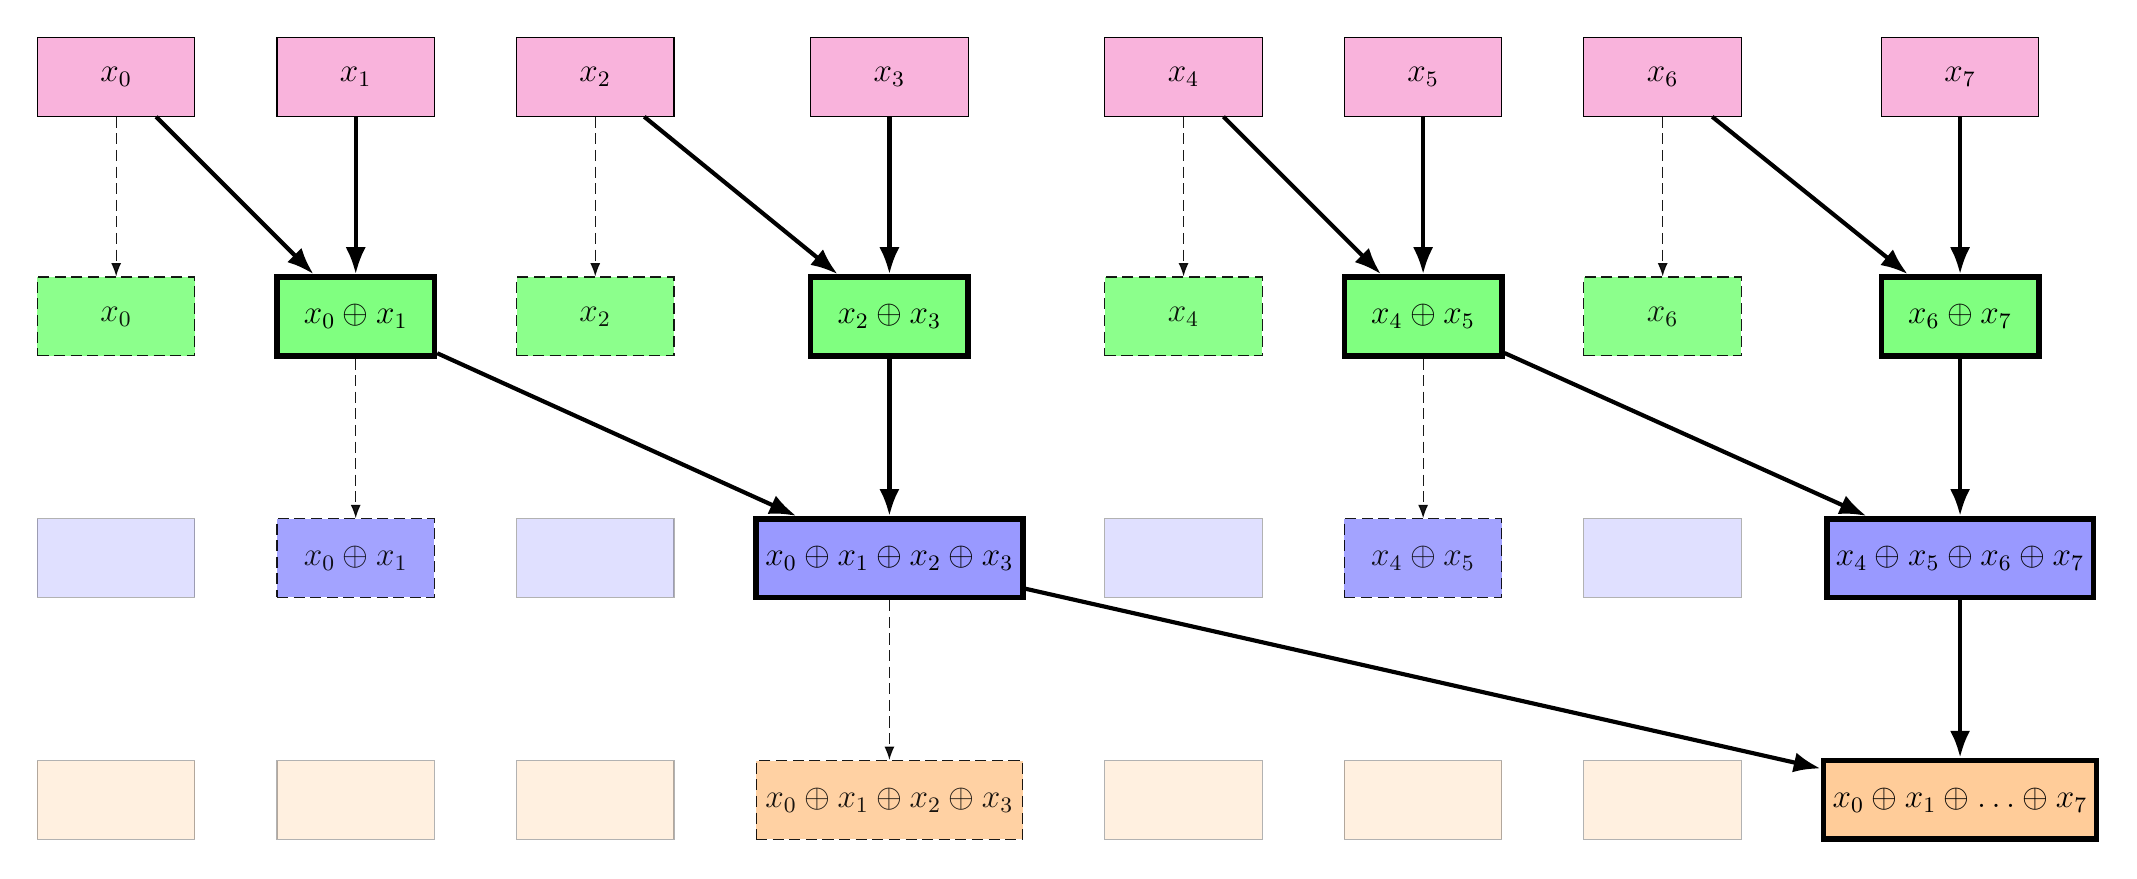
\begin{tikzpicture}[>=Latex]

\matrix[column sep=1cm, row sep=2cm] (m) {
  % Level 0
  \node[level0] (A0) {$x_0$}; &
  \node[level0] (A1) {$x_1$}; &
  \node[level0] (A2) {$x_2$}; &
  \node[level0] (A3) {$x_3$}; &
  \node[level0] (A4) {$x_4$}; &
  \node[level0] (A5) {$x_5$}; &
  \node[level0] (A6) {$x_6$}; &
  \node[level0] (A7) {$x_7$}; \\
  
  % Level 1 (distance 1)
  \node[level1,dashed] (B0) {$x_0$}; &
  \node[level1,newOp] (B1) {$x_0 \oplus x_1$}; &
  \node[level1,dashed] (B2) {$x_2$}; &
  \node[level1,newOp] (B3) {$x_2 \oplus x_3$}; &
  \node[level1,dashed] (B4) {$x_4$}; &
  \node[level1,newOp] (B5) {$x_4 \oplus x_5$}; &
  \node[level1,dashed] (B6) {$x_6$}; &
  \node[level1,newOp] (B7) {$x_6 \oplus x_7$}; \\
  
  % Level 2 (distance 2)
  \node[level2,transparent] (C0) {}; &
  \node[level2,dashed] (C1) {$x_0 \oplus x_1$}; &
  \node[level2,transparent] (C2) {}; &
  \node[level2,newOp] (C3) {$x_0 \oplus x_1 \oplus x_2 \oplus x_3$}; &
  \node[level2,transparent] (C4) {}; &
  \node[level2,dashed] (C5) {$x_4 \oplus x_5$}; &
  \node[level2,transparent] (C6) {}; &
  \node[level2,newOp] (C7) {$x_4 \oplus x_5 \oplus x_6 \oplus x_7$}; \\
  
  % Level 3 (distance 4)
  \node[level3,transparent] (D0) {}; &
  \node[level3,transparent] (D1) {}; &
  \node[level3,transparent] (D2) {}; &
  \node[level3,dashed] (D3) {$x_0 \oplus x_1 \oplus x_2 \oplus x_3$}; &
  \node[level3,transparent] (D4) {}; &
  \node[level3,transparent] (D5) {}; &
  \node[level3,transparent] (D6) {}; &
  \node[level3,newOp] (D7) {$x_0 \oplus x_1 \oplus \dots \oplus x_7$}; \\
};

% Draw arrows
\foreach \i/\j in {0/1,2/3,4/5,6/7} {
  \draw[->,line width=1.5pt] (A\i) -- (B\j);
  \draw[->,line width=1.5pt] (A\j) -- (B\j);
}
\draw[->,line width=1.5pt] (B1) -- (C3);
\draw[->,line width=1.5pt] (B3) -- (C3);
\draw[->,line width=1.5pt] (B5) -- (C7);
\draw[->,line width=1.5pt] (B7) -- (C7);
\draw[->,line width=1.5pt] (C3) -- (D7);
\draw[->,line width=1.5pt] (C7) -- (D7);

\draw[->, dashed] (A0) -- (B0);
\draw[->, dashed] (A2) -- (B2);
\draw[->, dashed] (A4) -- (B4);
\draw[->, dashed] (A6) -- (B6);
\draw[->, dashed] (B1) -- (C1);
\draw[->, dashed] (B5) -- (C5);
\draw[->, dashed] (C3) -- (D3);

\end{tikzpicture}
\end{document}
